\documentclass{standalone}
\usepackage{pgfplots}
\pgfplotsset{compat=newest}

\begin{document}
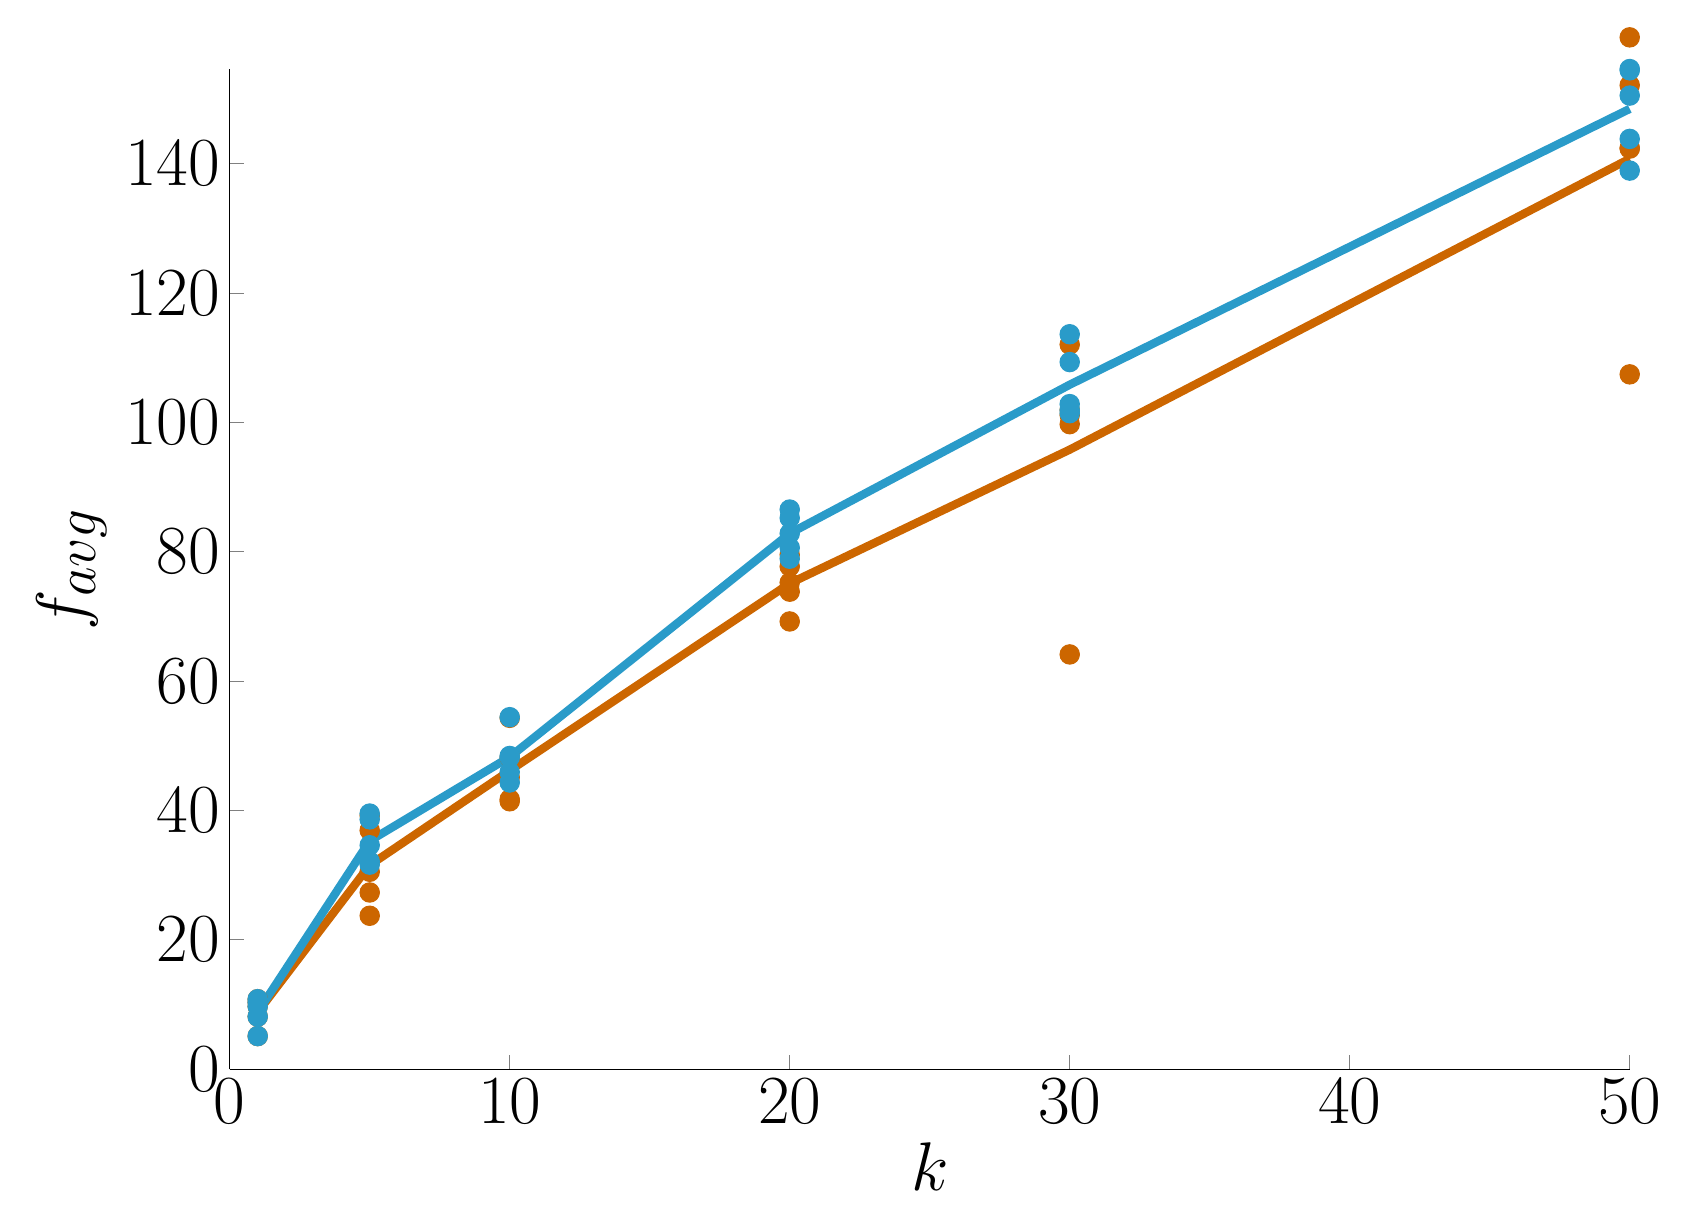
\begin{tikzpicture}

\begin{axis}[%
tick label style={font=\Huge},
label style={font=\Huge},
legend style={font=\Huge},
view={0}{90},
max space between ticks=50pt,
width=7in,
height=5in,
scale only axis,
xmin=0, xmax=50,
xtick={0, 10, 20, 30, 40, 50},
xlabel={$k$},
ymin=0, ymax=154.6,
%ytick={0, 200, 400, 600, 800, 1000},
ylabel={$f_{avg}$},
major tick length=5pt,
axis lines*=left,
legend cell align=left,
clip=false]

\addplot [
only marks,
mark=*,
mark size=3.5pt,
color=orange!80!black,
%solid,
%line width=2pt,
]
coordinates{
(1,5.1)(1,8.1)(1,9.7)(1,10.3)(1,10.8)(5,23.7)(5,27.3)(5,30.5)(5,36.9)(5,39.2)(10,41.4)(10,41.7)(10,45.1)(10,48.2)(10,54.3)(20,69.2)(20,73.8)(20,75.2)(20,77.7)(20,79.5)(30,64.1)(30,99.7)(30,101.1)(30,101.9)(30,112.0)(50,107.4)(50,142.3)(50,142.4)(50,152.1)(50,159.5)
};

\addplot [
only marks,
mark=*,
mark size=3.5pt,
color=cyan!80!black,
%solid,
%line width=2pt,
]
coordinates{
(1,5.1)(1,8.1)(1,9.7)(1,10.3)(1,10.8)(5,31.6)(5,32.1)(5,34.6)(5,38.6)(5,39.5)(10,44.3)(10,45.9)(10,48.2)(10,48.4)(10,54.4)(20,78.9)(20,80.6)(20,82.8)(20,85.2)(20,86.5)(30,101.4)(30,101.9)(30,102.8)(30,109.3)(30,113.6)(50,138.9)(50,143.8)(50,150.5)(50,154.4)(50,154.6)
};

\addplot [
color=orange!80!black,
solid,
line width=3pt
]
coordinates{
(1,8.8)(5,31.52)(10,46.14)(20,75.08)(30,95.76)(50,140.74)
};

\addplot [
color=cyan!80!black,
solid,
line width=3pt
]
coordinates{
(1,8.8)(5,35.28)(10,48.24)(20,82.8)(30,105.8)(50,148.44)
};


\end{axis}
\end{tikzpicture}
\end{document}
